%%%%%%%%%%%%%%%%%%%%%%%%%%%%%%%%%%%%%%%%%%%%
\documentclass[12pt]{article}
\usepackage[french]{babel}
\usepackage[T1]{fontenc}
\usepackage[utf8]{inputenc}
\usepackage{xcolor,times}
\usepackage{listings}
\usepackage{amsmath}
\usepackage{fancyhdr}
\usepackage{graphicx}
\usepackage{multicol}
\usepackage{verbatim}
\usepackage{url}

\pagestyle{fancy}
\lhead{CALIME Adrien - DENIS Alexandre}
\rhead{TP3 aide à la décision}

\title{\Huge{Compte-rendu du TP3 d'aide à la décision : Le VRPTW}\vspace{2\baselineskip} \\\ 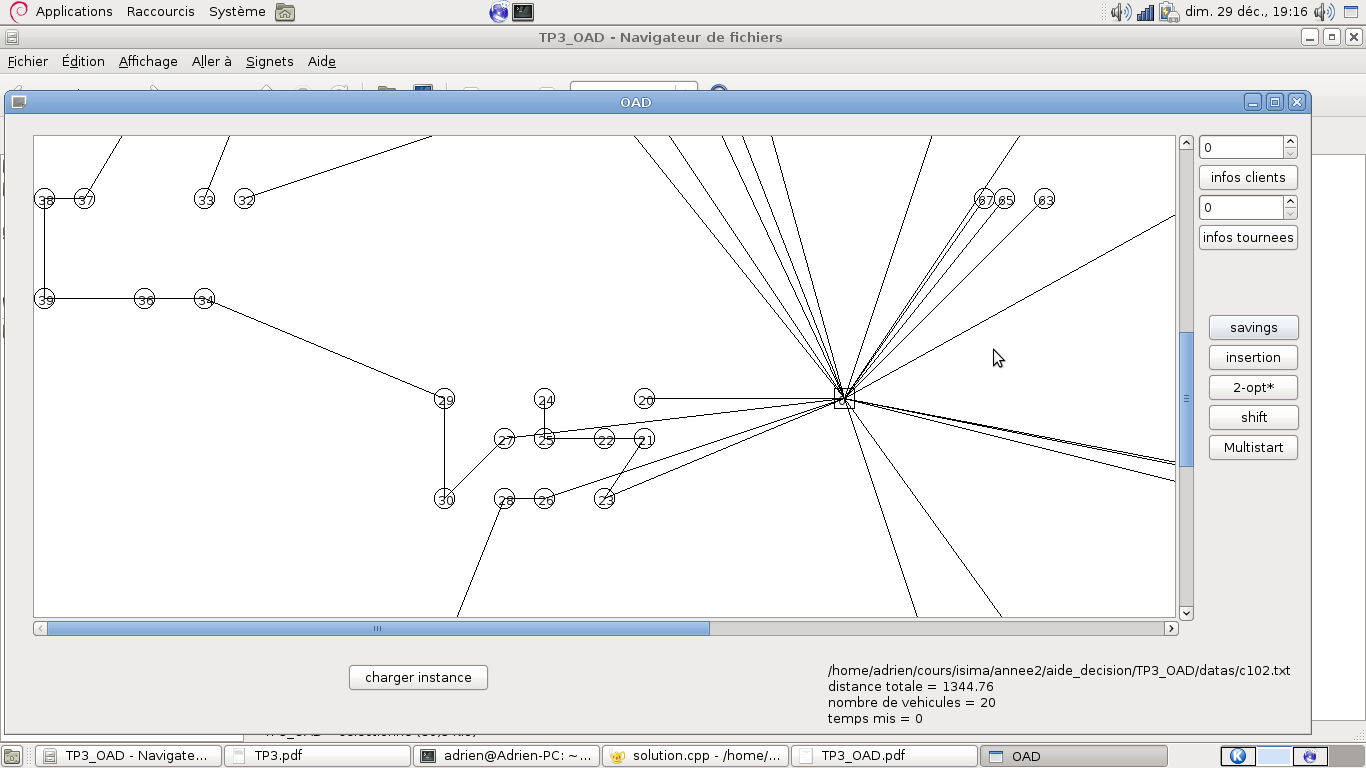
\includegraphics[width=15cm,height=10cm]{Capture.png}   \\\ }

\author{CALIME Adrien - DENIS Alexandre (F2)}
\date{}

\newcommand*\styleC{\fontsize{9}{10pt}\usefont{T1}{ptm}{m}{n}\selectfont }
\newcommand*\styleD{\fontsize{9}{10pt}\usefont{OT1}{pag}{m}{n}\selectfont }

\makeatletter
% on fixe le langage utilisé
\lstset{language=c}
\edef\Motscle{emph={\lst@keywords}}
\expandafter\lstset\expandafter{%
  \Motscle}
\makeatother


\definecolor{Ggris}{rgb}{0.45,0.48,0.45}

\lstset{emphstyle=\rmfamily\color{blue}, % les mots réservés de matlab en bleu
basicstyle=\styleC,
keywordstyle=\ttfamily,
commentstyle=\color{Ggris}\styleD, % commentaire en gris
numberstyle=\tiny\color{red},
numbers=left,
numbersep=10pt,
lineskip=0.7pt,
showstringspaces=false}
%  % inclure le fichier source
\newcommand{\FSource}[1]{%
\lstinputlisting[texcl=true]{#1}
}

%%%%%%%%%
\textwidth=15cm
\textheight=21cm
%\hoffset=-2.5cm
\tolerance=9000
\hbadness=9000
\pretolerance=2500

\begin{document}

\maketitle

\clearpage
%\renewcommand{\contentsname}{\\\rule{\linewidth}{2pt}\\\hspace*{\stretch{1}}Table des matières\hspace*{\stretch{1}}\\\rule{\linewidth}{2pt}\\\\}
\tableofcontents

\clearpage
\section{Introduction}\vspace{2\baselineskip}

\paragraph{}
Dans ce TP, le but est de représenter le problème du VRPTW à partir d'un fichier et d'écrire des algorithmes pour optimiser ce type de problème. 
Le problème du VRPTW, pour Vehicle Routing Problem with Time Windows, désigne le fait d'accéder à toute une liste de clients le plus rapidement 
possible tout en respectant leurs délais à partir d'un point donné.
\\

\paragraph{}
Les algorithmes ont été écrits en C++, langage proposé par M.Duhamel. Dans ces algorithmes, il y avait : \\\
\begin{itemize}
  \item Création d'une instance d'un VRPTW à partir d'un fichier.
  \item Création d'un premier chemin avec des heuristiques de construction telles que l'algorithme de Savings et l'algorithme d'Insertion.
  \item Optimisation de la situation avec des heuristiques comme le 2-opt* ou le shift.
  \item Optimisation de la situation via un algorithme appelé le multi-start.\\
\end{itemize}

\paragraph{}
En plus de ces algorithmes, quelques fonctionnalitées ont été ajoutées afin de rendre le travail plus représentatif. En effet, nous avons une interface 
graphique réalisée en QT permettant de visualiser l'ensemble des clients et des routes à prendre d'un problème que l'on peut choisir soi-même dans le
dossier adéquat. De plus, il est possible de consulter à tout moment des informations concernant les clients et les tournées. Puis, le logiciel donne 
aussi la possibilité de lancer l'algorithme de son choix sur l'instance choisie.

\paragraph{}
Les algorithmes cités avant seront tout d'abord décrits dans leur globalité. Puis, nous aborderons l'aspect technique de ces algorithmes. Enfin, 
nous effectuerons une étude sur la performance de l'algorithme multi-start.

\clearpage
\section{Description des points nécessaires à l’optimisation d’un VRPTW}

\subsection{Evaluation d'une solution}

\paragraph{}
Afin de créer notre graphe de départ, on a avant tout étudié le format du fichier de lecture que l'on a modifié afin de faciliter 
sa lecture. Nous avons donc un format de fichier de la forme suivante : \\

\begin{tabular}{ *{8}{c} }
   ligne 1 : & capacité véhicules &  & & & & &\\
   ligne 2 : & num client & X & Y & demande & ouverture & fermeture & temps service \\
   ... & & & & & & & \\
   ligne n : & num client & X & Y & demande & ouverture & fermeture & temps service \\
 \end{tabular}

\paragraph{}
Après compréhension du format du fichier, il ne restait plus qu'à lire ses données. La lecture est simple, il suffit de récupérer la capacité 
des véhicules puis pour chaque ligne de créer un client ayant les caractéristiques de la ligne lue. Cette lecture s'est faite via une variable de
type \textbf{fstream}, ainsi on a un flux sur le fichier permettant une lecture rapide et efficace du fichier.

\paragraph{}
Après lecture du fichier, il est nécessaire d'initialiser la solution. Pour ce faire, nous avons utilisé les heuristiques d'Insertion et de Savings.

\subsection{L'heuristique d'Insertion}

\paragraph{}
Cette heuristique permet de créer une solution initiale au problème. Le but de cet algorithme est de créer des tournées les unes après à les autre en 
ajoutant les clients les uns après les autres avec des critères bien définis.

\paragraph{}
Le but est donc de créer au départ une tournée vide puis d'ajouter, un par un, les meilleurs clients. Meilleur est un terme subjectif car, on peut choisir les 
clients selon un ordre défini. Mais le terme meilleur désigne le client qui augmente le moins la distance totale de la tournée.

\paragraph{}
Puis, lorsqu'on ne peut plus ajouter de client à la tournée, on clôture la tournée et on en recréé une nouvelle. Lorsque tous les clients ont été traités 
dans les tournées alors l'algorithme s'arrête.

\paragraph{}
On a donc maintenant une solution initiale faite à partir de l'insertion du meilleur client possible. 

\paragraph{}
Après avoir vu dans sa généralité l'Insertion, nous allons nous pencher sur Savings.

\subsection{L'heuristique Savings}

\paragraph{}
A l'inverse de l'heuristique précedente, Savings commence tout d'abord par créer un nombre de tournées égal au nombre de clients. C'est à dire que l'on a un 
client pour une tournée.

\paragraph{}
Puis après la création de ces tournées avec client unique, Savings permet de fusionner des tournées. Pour ce faire, Savings compare les gains apportés par 
toutes les fusions possibles et prend le gain le plus conséquent. Ainsi, petit à petit, cet heuristique fusionne les différentes tournées afin d'en 
réduire un maximum.

\paragraph{}
Cette comparaison de gains se fait via un stockage des différents arcs possibles à créer suivi d'un triage en fonction de leurs gains. Ainsi, il suffit de récupérer 
le gain proposé par le premier arc stocké dans la liste.

\paragraph{}
Cette opération se fait autant de fois que possible afin de réduire au maximum les tournées et la distance totale du VRPTW. On a donc maintenant une solution 
initiale prête à être améliorée.

\subsection{L'amélioration par le 2-opt*}

\paragraph{}
L'algorithme 2-opt* est une heuristique permettant d'améliorer la solution par l'échange de fin de tournée. C'est à dire que l'on choisit deux arcs de deux 
tournées différentes dont on échange les extrémités sortantes de ces arcs.

\paragraph{}
Cette amélioration permet aussi la supression d'une tournée. En effet, si les arcs à échanger correspondent à une fin de tournée et à un début de tournée 
alors il y a concaténation de ces deux tournées afin d'en avoir plus qu'une au lieu de deux.

\paragraph{}
Evidemment, lors du test des arcs à échanger, certains cas ne sont pas à prendre en compte. En effet, si deux arcs sont en début de tournée, aucun changement ne 
sera apporté à la solution, de même si nous avons deux arcs en fin de tournées. Donc, afin de ne pas perdre de temps, on ne teste pas ces types de 
cas inutiles.

\paragraph{}
Cet algortihme n'est pas le seul qui existe pour améliorer une solution de type VRPTW, il en existe d'autres telles que le shift que nous avons implémenté.

\subsection{L'amélioration par le shift}

\paragraph{}
Cet heuristique d'insertion s'opère seulement au sein d'une tournée. Elle permet d'optimiser la solution uniquement sur les tournées elles-mêmes.

\paragraph{}
Pour améliorer, cette heuristique commence par prendre un sommet et regarde si ce sommet peut améliorer la solution s'il est placé à un autre endroit 
dans cette tournée. Puis, on refait ce test avec tous les autres sommets de la tournée. 

\paragraph{}
A la fin des différents tests, le sommet qui sera déplacé sera celui qui améliore le plus la solution. Ainsi de suite, on continue ces opérations 
jusqu'à que l'on ne puisse plus améliorer la solution.

\paragraph{}
Nous avons vu quels sont les procédés pour créer et améliorer une solution de type VRPTW, nous allons maintenant voir un algorithme permettant 
d'automatiser tous les procédés vus afin d'essayer de trouver la solution optimale.

\subsection{Le multi-start}

\paragraph{}
Le multi-start est un algorithme permettant d'être le plus proche possible de la solution optimale. 

\paragraph{}
Pour ce faire, il commence à initialiser une solution puis à effectuer une recherche locale dessus. Puis, il recommence l'opération autant de fois 
que souhaité par le développeur afin de continuer à chercher d'autres solutions qui pourraient être meilleures.

\paragraph{}
L'initilisation se fait via les algorithmes permettant la création de la solution que nous avons vu avant. La recherche locale s'effectue avec du 2-opt* 
et du shift alternés afin de descendre le plus bas possible dans l'optimum de la solution.

\paragraph{}
Le multi-start se termine en gardant la meilleure solution trouvée grâce à l'utilisation de tous les algorithmes présentés.

\paragraph{}
Après avoir étudié dans l'aspects général les heuristiques utilisées, nous allons les étudier plus en détails grâce à leurs algorithmes.

\clearpage
\section{Description des algorithmes}

\subsection{Insertion}

\begin{tabbing}
\hspace{1cm} \= \hspace{1cm} \= \kill
01  Tant que tous les clients ne sont pas dans une tournée\\
02  \> Si il faut recréer une tournée\\
03  \> \> Initialiser une tournée vide \\
04  \> Fin si\\
05  \> Pour chaque client\\
06  \> \> Si il respecte les contraintes de capacité et les fenêtres de temps \\
07  \> \> \ \ \ \ \ \ \ \ \ \ \ \ Calculer son gain\\
08  \> \> \ \ \ \ \ \ \ \ \ \ \ \ Si le gain calculé est meilleur alors on garde ce client \\
09  \> \> Fin si \\
10  \> Fin pour \\
11  \> Si un meilleur client a été trouvé \\
12  \> \> Insérer le client à la fin de la tournée courante\\
13  \> Sinon \\
14  \> \> Mettre le booléen de création d'une tournée vide à vrai \\
15  \> Fin si \\
16  Fin tant que \\
\end{tabbing}

\subsection{Savings}

\begin{tabbing}
\hspace{1cm} \= \hspace{1cm} \= \kill
01  Pour chaque client\\
02  \> Créer une tournée vide comportant le client courant\\
03  Fin pour\\
04  Pour chaque client\\
05  \> Pour chaque client\\
06  \> \> Ajouter l'arc reliant ces deux clients à la liste des arcs \\
07  \> Fin pour \\
08  Fin pour \\
09  Trier les arcs par leurs gains \\
10  Pour chaque arc \\
11  \> Si les deux arcs ne sont pas dans la même tournée \\
12  \> \> Si il y a concaténation et respect des contraintes (capacités et TW)\\
13  \> \> \ \ \ \ \ \ \ \ \ \ \ \ Fusionner les deux tournées via l'arc courant \\
14  \> \> Fin si \\
15  \> Fin si \\
16  Fin Pour \\
17  Supprimer les tournées vides issues des fusions \\
\end{tabbing}

\subsection{2-opt*}

\begin{tabbing}
\hspace{1cm} \= \hspace{1cm} \= \kill
01  Tant qu'on peut améliorer\\
02  \> Pour chaque arc de chaque tournée\\
03  \> \> Pour chaque arc de chaque tournée \\
04  \> \> \ \ \ \ \ \ \ \ \ \ \ \ Si les contraintes sont respectées avec un gain améliorant \\
05  \> \> \ \ \ \ \ \ \ \ \ \ \ \ \ \ \ \ \ \ \ \ \ \ \ \ Echanger les fins de tournées\\
06  \> \> \ \ \ \ \ \ \ \ \ \ \ \ Fin si \\
07  \> \> Fin pour \\
08  Fin pour \\
\end{tabbing}

\paragraph{}
Dans cet algorithme, quand on parle de contraintes respectées, on parle de tester les cas inutiles cités au 2.4 et les tests de capacités ainsi que les fenêtres
de temps. Les tests effectués sont réalisés sur tous les clients qui seront échangés afin de savoir si chaque client pourra être changé de tournée.

\subsection{Shift}

\begin{tabbing}
\hspace{1cm} \= \hspace{1cm} \= \kill
01  Pour chaque tournée possédent au moins deux clients\\
02  \> Tant qu'on peut améliorer la tournée\\
03  \> \> Pour chaque client de la tournée \\
04  \> \> \ \ \ \ \ \ \ \ \ \ \ \ Calculer une meilleure position possible \\
05  \> \> \ \ \ \ \ \ \ \ \ \ \ \ Si la position calculée est la meilleure\\
06  \> \> \ \ \ \ \ \ \ \ \ \ \ \ \ \ \ \ \ \ \ \ \ \ \ \ Conserver le client courant et la position calculée\\
07  \> \> \ \ \ \ \ \ \ \ \ \ \ \ Fin si \\
08  \> \> Fin pour \\
09  \> \> Si il existe une amélioration \\
10  \> \> \ \ \ \ \ \ \ \ \ \ \ \ Déplacer le client retenu à la position retenue avant \\
11  \> \> Fin si \\
12  \> Fin tant que \\
13  Fin pour \\
\end{tabbing}

\paragraph{}
Le calcul de la meilleure position possible se fait via une boucle parcourant le reste de la tournée. Lors de ce parcours, on regarde si la position 
permet à la solution d'être améliorée.

\subsection{Multi-start}

\begin{tabbing}
\hspace{1cm} \= \hspace{1cm} \= \kill
01  Pour un nombre d'itérations défini\\
02  \> Construire une solution randomisée à l'aide d'une heuristique de construction\\
03  \> Effectuer une recherche locale \\
04  \> Si c'est la meilleure solution \\
05  \> \> On la conserve\\
06  \> Fin si\\
07  Fin pour\\
08  Conserver et appliquer la meilleure solution trouvée.\\
\end{tabbing}

\paragraph{}
La recherche locale se fait grâce à une succession de 2-opt* et de shift répétée juqu'à ne plus pouvoir améliorer la solution.


\paragraph{}
Nous avons vu les différents algorithmes par leurs fonctionnements et leurs implémentations. Nous allons donc maintenant effectuer une étude de performance sur 
le programme que nous avons conçu.

\clearpage
\section{Etude de performances de l'algorithme multi-start}
L'étude du programme se fera via la fonction multi-start car c'est cette fonction qui fait tournée le programme. Nous effectuerons l'étude grâce aux tableaux 
fournis en annexe du sujet. Les valeurs rentrées dans le tableau ont réalisées pour 10 itérations du multi-start.\\\

\begin{tabular}{ |*{4}{c|} }
\hline
   Instance & Nombre de véhicules & Distance & Temps mis \\
 \hline
   c101 & 20 & 1332.95 & 5s \\
 \hline
   c102 & 16 & 1176.56 & 3s \\
 \hline
   c104 & 8 & 1119.44 & 0s \\
 \hline
   c106 & 13 & 1256.93 & 2s \\
 \hline
   c201 & 6 & 800.41 & 1s \\
 \hline
   c203 & 4 & 968.54 & 1s \\
 \hline
   c205 & 4 & 786.38 & 1s \\
 \hline
   c207 & 3 & 1057.7 & 0s \\
 \hline
   r203 & 2 & 1061.6 & 0s \\
 \hline
   r204 & 2 & 888.73 & 0s \\
 \hline
   r207 & 2 & 1061.6 & 0s \\
 \hline
   r209 & 3 & 1136.64 & 0s \\
 \hline
   r211 & 2 & 952.54 & 0s \\
 \hline
   rc201 & 2 & 1537.41 & 0s \\
 \hline
   rc203 & 4 & 1399.3 & 0s \\
 \hline
   rc205 & 2 & 1272.63 & 0s \\
 \hline
   rc208 & 2 & 1011.48 & 0s \\
 \hline
 \end{tabular}

\paragraph{}
Ce tableau nous fait tout d'abord remarquer que les temps de calculs sont extrêmement courts. Seulement, les meilleures distances atteintes par notre 
programme sont toujours au-dessus de celles proposées sur le site \textbf{http://www.sintef.no/Projectweb/TOP/VRPTW/Solomon-benchmark/100-customers/}.
De plus, lors de l'exécution du programme, nous pouvons remarquer qu'un certain nombre d'instances font échouer le programme. 

\paragraph{}
Pour finir cette partie, les algorithmes que nous avons implémentés nous donne des résultats à peu près convenable pour des délais très courts sur 
les solutions compatibles à notre programme.

\clearpage
\section{Conclusion}

\paragraph{}
Ce TP nous a permis d'élargir nos connaissances dans le domaine de la recherche opérationnelle. En effet, nous avons pu concevoir des algortihmes que nous 
connaissions seulement de nom. On a ainsi compris plus en détail à quoi servaient ces algorithmes.

\paragraph{}
De plus, par le biais des nombreuses heures que nous avons passées sur le programme, nous avons pu étendre nos connaissances dans la programmation objet en C++.

\paragraph{}
Nous avons donc pu concevoir un programme pouvant traiter les problèmes de VRPTW donnant des résultats, certes pas exceptionels, mais que l'on peut juger de convenables.

\paragraph{}
Seulement, des problèmes subsistent dans le logiciel, et ce malgré les heures de débuggage que nous avons passées dessus. En effet, pour un 
certain nombres d'instances, le programme ne fonctionne pas. 


\end{document}